\documentclass[12pt,a4paper]{beamer}
\usetheme{Darmstadt}
\usepackage[utf8]{inputenc} 
\usepackage{ngerman}
%\usepackage[applemac]{inputenc}

\usepackage[T1]{fontenc}

% Official title from the 283-Fahrplan, looks kinda stupid this way
\title[Open-GWAS]{Was die Post-Genomics-\"Ara f\"ur die Privatsph\"are bedeutet}%\\Freeing Genetic Data from Corporate Vaults}
% short title in [], long in {}
\date{29.12.2011}
\author{Bastian Greshake and Philipp Bayer}

\setbeamertemplate{navigation symbols}{} % get rid of unused symbols

\begin{document}
\begin{frame}
\titlepage
\end{frame}

\begin{frame}{Overview}
\tableofcontents
\end{frame}

% The sections still have stupid names
\section{A short history of Genomics}
\subsection{In the beginning...}

\begin{frame}{DNA?}
	\begin{itemize}
		\item Rezept zur Kopienerzeugung
		\pause \item Struktur 1953 entschl\"usselt (Watson \& Crick)
		\begin{center}
			
\includegraphics[scale=0.3]{220px-DNA_simple.png} \\
		\end{center}
	\end{itemize} 
\end{frame}

\begin{frame}{DNA Sequenzierungen?}
	\begin{center}
	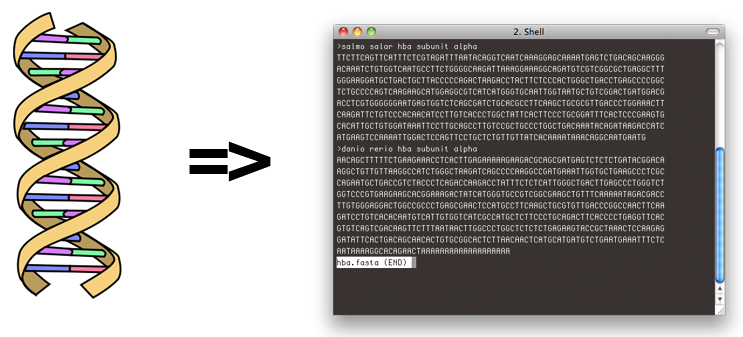
\includegraphics[scale=0.4]{dna_to_text.jpg} \\
	\end{center}
	\begin{itemize}
		\item Lesbarmachen der Basen-Abfolge
		\pause \item Erste benutzbare Methode: 1977 von Frederick Sanger
		\pause \item Im gleichen Jahr: Erstes Genom (von Bakteriophage PhiX174) komplett sequenziert (5386bp).
	\end{itemize}
\end{frame}

\subsection{Modern Genomics}

\begin{frame}{Das Human Genome Project}
	\begin{itemize}
		\item Start: 1990
		\pause \item Abschluss: 2001
		\pause \item Kosten: \~\ \$3 Milliarden 
	\end{itemize}
\end{frame} 

\begin{frame}{Weitere Humangenomik}
	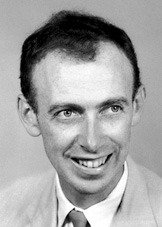
\includegraphics[scale=0.4]{watson.jpg}
	\begin{itemize}
		\item 2008: Genom von James Watson komplett sequenziert
		\begin{itemize}
			\pause \item In 2 Monaten
			\pause \item \~\ 3 Millionen USD
		\end{itemize}
	\end{itemize}
\end{frame}

\begin{frame}{Heute}
	\begin{itemize}
		\item Kosten f\"ur komplettes, menschliches Genom: \~\ USD 10.000
		\item Menschliches Exom (alle in Protein \"ubersetzten Bereiche): USD 999  
		\item Direct-To-Customer (DTC) Gen-Analysen: \~\ USD 99
	\end{itemize}
\end{frame}

\section{Aktueller Nutzen und Missbrauch?}

\subsection{Allgemeines}

\begin{frame}{Gesundheit}
	\begin{itemize}
		\item Risikoeinsch\"atzung (Alzheimer, Parkinsons, Krebsarten...)
		\pause \item \"Ubertr\"ager von Erbkrankheiten? (H\"amochromatose)
		\pause \item Pharmakogenomik 
	\end{itemize}
\end{frame}

\begin{frame}{Forensik}
	\begin{itemize}
		\item DNA Fingerprinting
		\pause \item Vorhersage von Merkmalsausprägungen (Haar- \& Augenfarbe) 
		\pause \item Vaterschaftstests / Genealogie
	\end{itemize}
\end{frame}

\begin{frame}{Personalisierte Werbung?}
	\begin{itemize}
		\item 2011: VISA reicht Patent für personalisierte Werbung aufgrund von genetischen Informationen ein
		\pause \item Allerdings noch nicht umgesetzt
	\end{itemize}
\end{frame}

\subsection{Öffentliche Daten} 

\begin{frame}{DTC Gentests}
	\begin{itemize}
		\item 23andMe hat über 100.000 Kunden
		\pause \item Immer mehr davon veröffentlichen ihre Daten im Netz
	\end{itemize}
	\begin{center}
		Nebenwirkungen?
	\end{center}
\end{frame}

\begin{frame}{Nebenwirkungen}	
	\begin{itemize}
		\item Erlaubt Open Science auf verschiedenen Plattformen
		\begin{itemize}
			\item Genomera / DIYgenomics
			\item openSNP
		\end{itemize}
		\pause \item Austausch zwischen \glqq Betroffenen\grqq und \glqq Experten\grqq
	\end{itemize}
\end{frame}

\begin{frame}{Nebenwirkungen}
	\begin{itemize}
		\item Diskriminierungspotential
		\begin{itemize}
			\item Arbeitgeber
			\item Versicherer
			\item ...
		\end{itemize}
		\pause \item Personalisierte Werbung (siehe \emph{VISA})
		\pause \item Wissen über genetische Variation ist nicht statisch
		\pause \item Genetische Informationen verraten mehr über Verwandte als ihnen vielleicht recht
	\end{itemize}
\end{frame}

\section{Fallbeispiele}
\subsection{Ein Nobelpreis ist keine Garantie...}
\begin{frame}{James Watson}
	\begin{itemize}
		\item Mutmaßlich Träger einer APOE4-Variante
		\pause \item Variante assoziiert mit Late Onset Alzheimers
		\pause \item Watsons Genom an der entsprechenden Stelle geschwärzt
	\end{itemize}
	\begin{center}
		\pause Wenige Monate nach Veröffentlichung...
	\end{center}
\end{frame}

\begin{frame}{James Watson}
	\begin{center}
		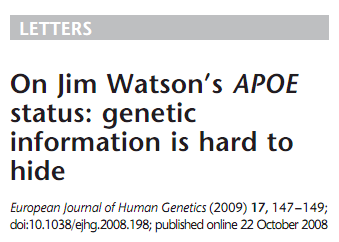
\includegraphics[scale=0.5]{watson_paper.png}
	\end{center}
	\begin{center}
		Genotype Imputation: \emph{Security through Obscurity} funktioniert nicht
	\end{center}
\end{frame}

\subsection{Sorry, Kids}
\begin{frame}{@gedankenstuecke und Verwandte}
	Durch Veröffentlichung meiner DTC-Ergebnisse ist nachvollziehbar: 
	\begin{itemize}
		\pause \item Meine Eltern \& Kinder haben (leicht) erhöhte Risiken für:
		\begin{itemize}
			\pause \item Rheumatoide Arthritis
			\pause \item Morbus Basedow
			\pause \item Morbus Crohn
			\pause \item Brustkrebs
			\pause \item Prostatakrebs
			\item ...
		\end{itemize} 
	\end{itemize}	
\end{frame}

\section{Die Zukunft}
\begin{frame}{Selbst Schuld?}
	\begin{center}
	\textbf{Wer sein Genom frei zugänglich macht, der muss sich ja auch nicht wundern(?)}
	\end{center}	
\end{frame}

\subsection{DNA lacht über dein Moore's Law}
\begin{frame}
	\begin{center}
		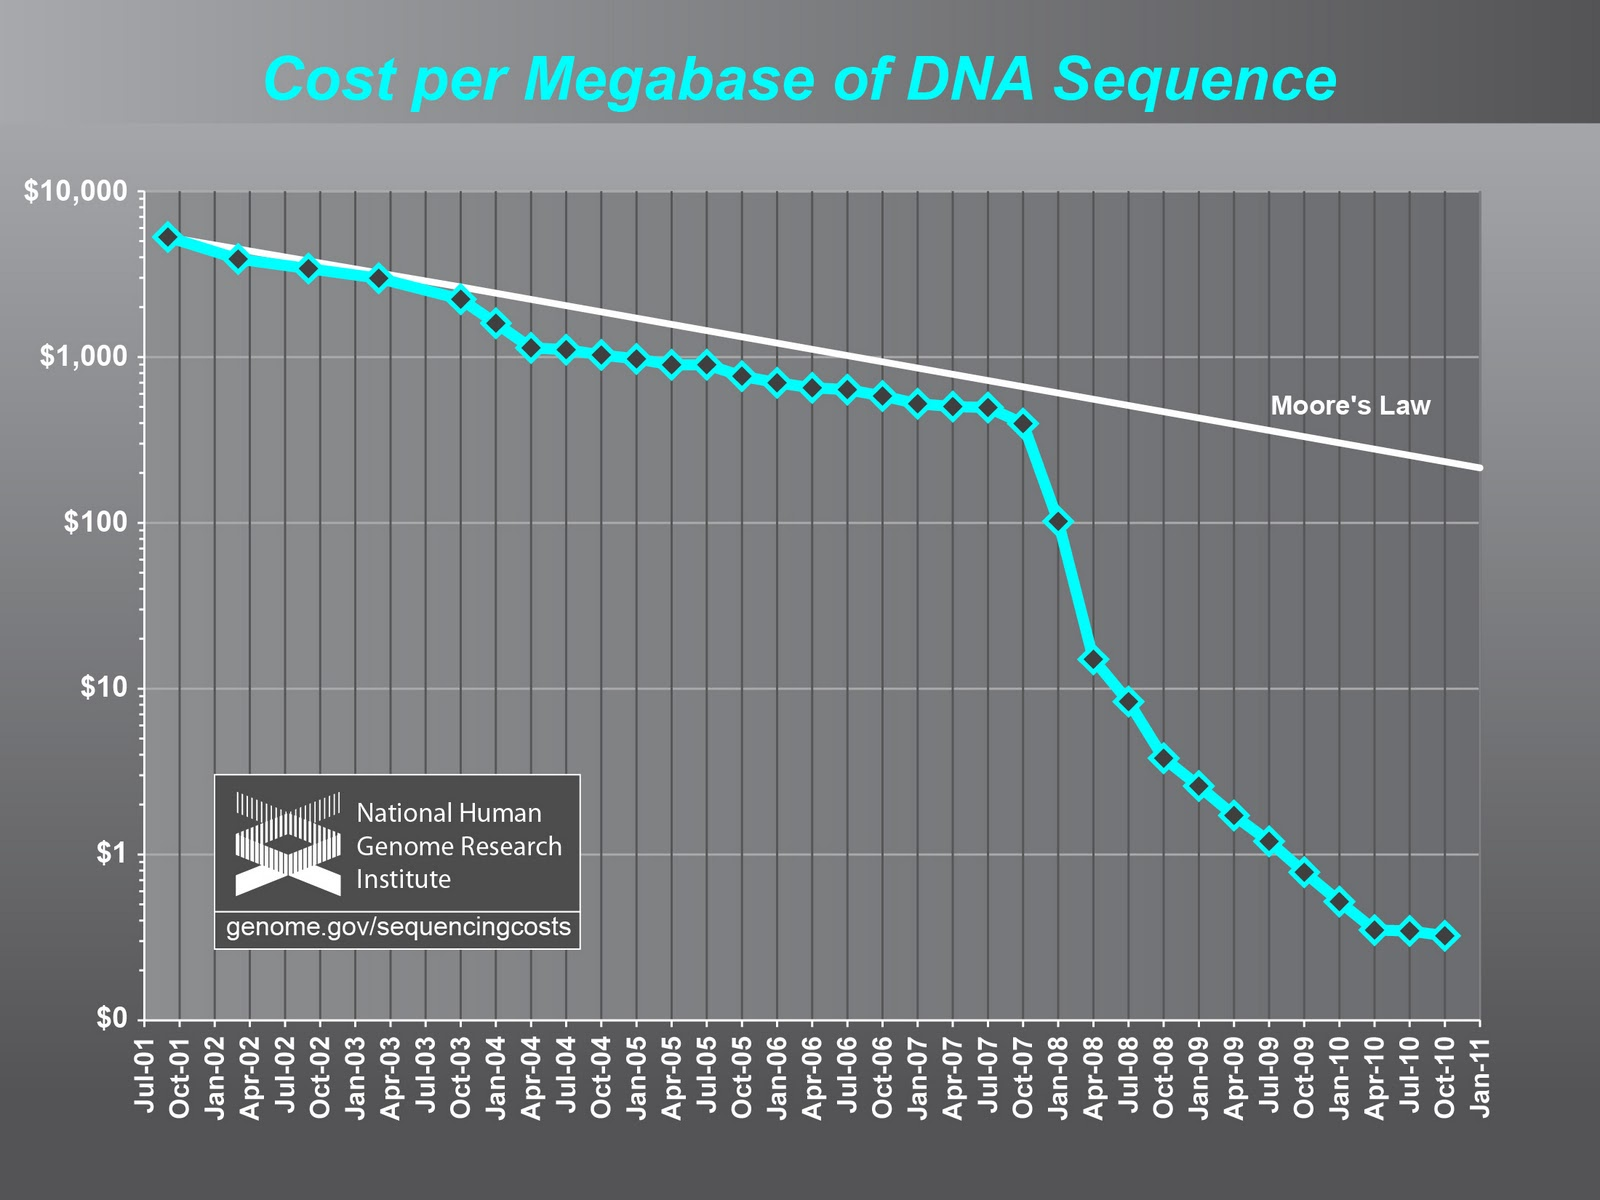
\includegraphics[scale=0.2]{moore.jpg}
	\end{center}
\end{frame}

\begin{frame}{Verfügbarkeit von gen. Daten}
	\begin{itemize}
		\item 2012/2013: 1000 Dollar-Genome 
		\pause \item Preise für DTC-Tests fallen ebenfalls (von 1000 auf 100 in 5 Jahren)
		\pause \item Genomsequenzierungen werden üblich bei medizinischen Untersuchungen
	\end{itemize}	
\end{frame}

\begin{frame}{DNA is here to stay}
	\begin{itemize}
		\item Eine Frage der Zeit bis von jedem DNA verfügbar ist
		\pause \item DTC-services können nicht überprüfen von wem eingesendete Proben stammen
		\pause \item Neue biologische Methoden finden neue Zusammenhänge 
	\end{itemize}
\end{frame}

\begin{frame}{Ein Beispiel}
	\begin{center}
		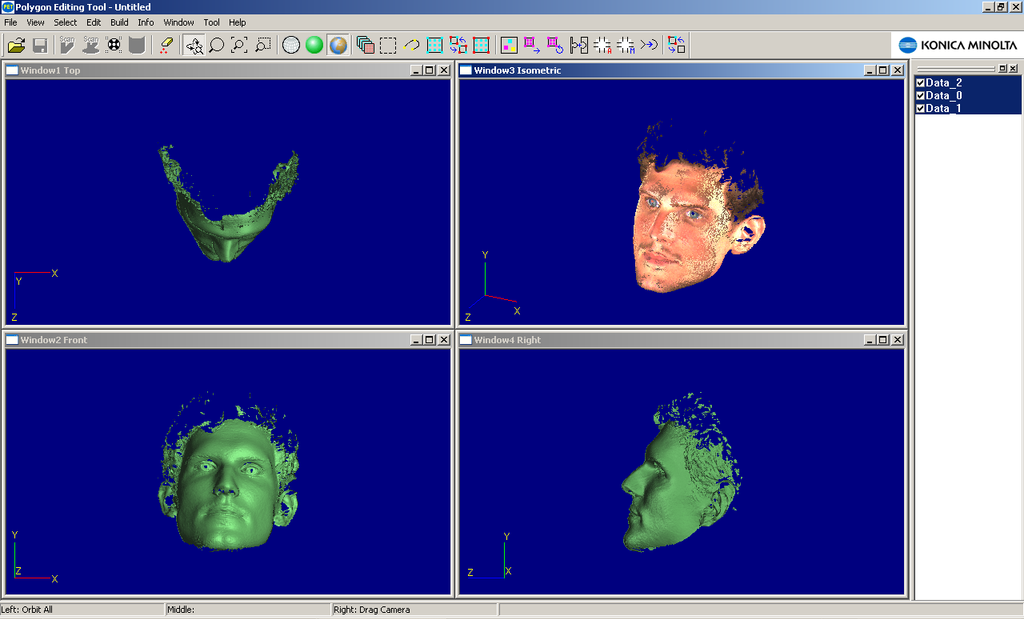
\includegraphics[scale=0.30]{head.png}
	\end{center}
	
\end{frame}

\section{The End}
\subsection{ATG...}
	\begin{frame}{Zusammenfassung}
		\begin{itemize}
			\item DNA von/für alle wird kommen
			\item Veröffentlichungen der Daten haben Nebenwirkungen
			\item Die Frage ist: Wie geht man damit um? 
			\item Bringen Gesetze hier etwas? (GINA, GenDG)
		\end{itemize}
	\end{frame}

\begin{frame}{...TGA}
	\begin{center}
		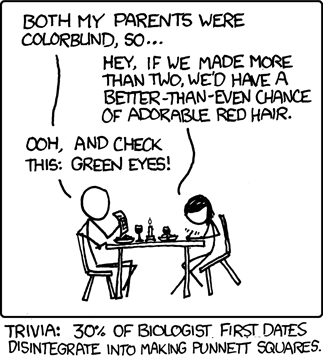
\includegraphics[scale=0.41]{xkcd.png}
		
		Vielen Dank! 
	\end{center}
\end{frame}
\end{document}
